\chapter[Story Board]{Story Board}

Esse story Board tem como  usuários principais pessoas que planejam suas viagens e que preferem pesquisar os preços das passagens áreas com antecedência. Diversas companhias áreas fazem promoções aos finais de semana geralmente de madrugada, isso faz com que a pessoa interessada tenham que ficar até tarde acordada no final de semana para conseguir achar passagens com preços em conta. Para os usuários que tem o habito de dormir cedo essa tarefa torna-se desgastante, pois para ele ter um panorama dos preços terá que abdicar de alguns finais de semana para realizar essa pesquisa. 

Com uma aplicação que possa ser configurada para trazer essa informação o usuário não terá mais que  despender esse esforço. A proposta do aplicativo é permitir que a pessoa insira a URL do site em que deseja fazer a pesquisa, a data e hora que ela deseja que a pesquisa seja realizada, informe dos valores limites desejáveis das passagens e quando o preço estiver dentro do estipulado o sistema irá notificá-lo. 

A figura abaixo apresenta uma pessoa que está realizando a pesquisa dos preços das passagens diversos  dias e horários, na sequência, tem o usuário preocupado pois deveria estar procurando por preços mais em conta até que um dia apresentam esse aplicativo para ele e a partir dai ele pode ir dormir feliz e sem preocupações.


\begin{figure}[h]
	\centering
	\label{fig01}
		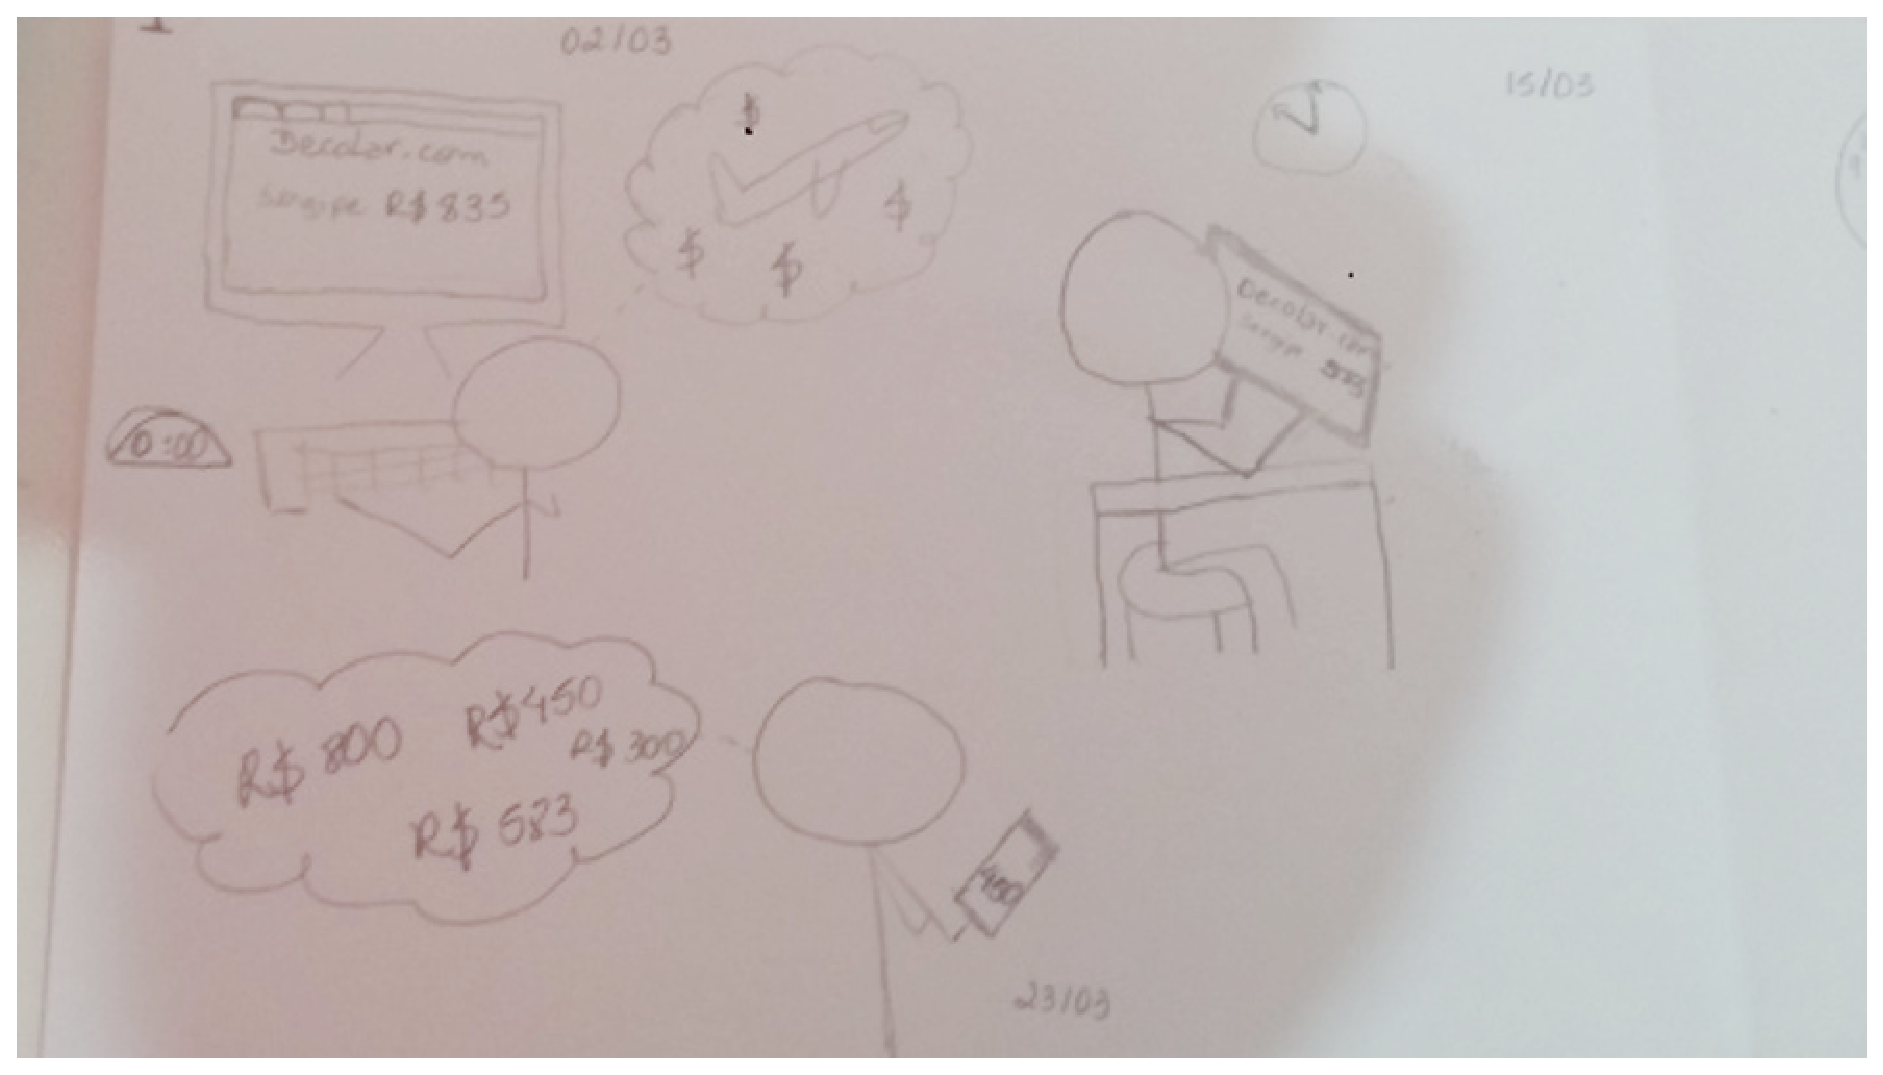
\includegraphics[keepaspectratio=true,scale=0.3]{figuras/quadro1.eps}
		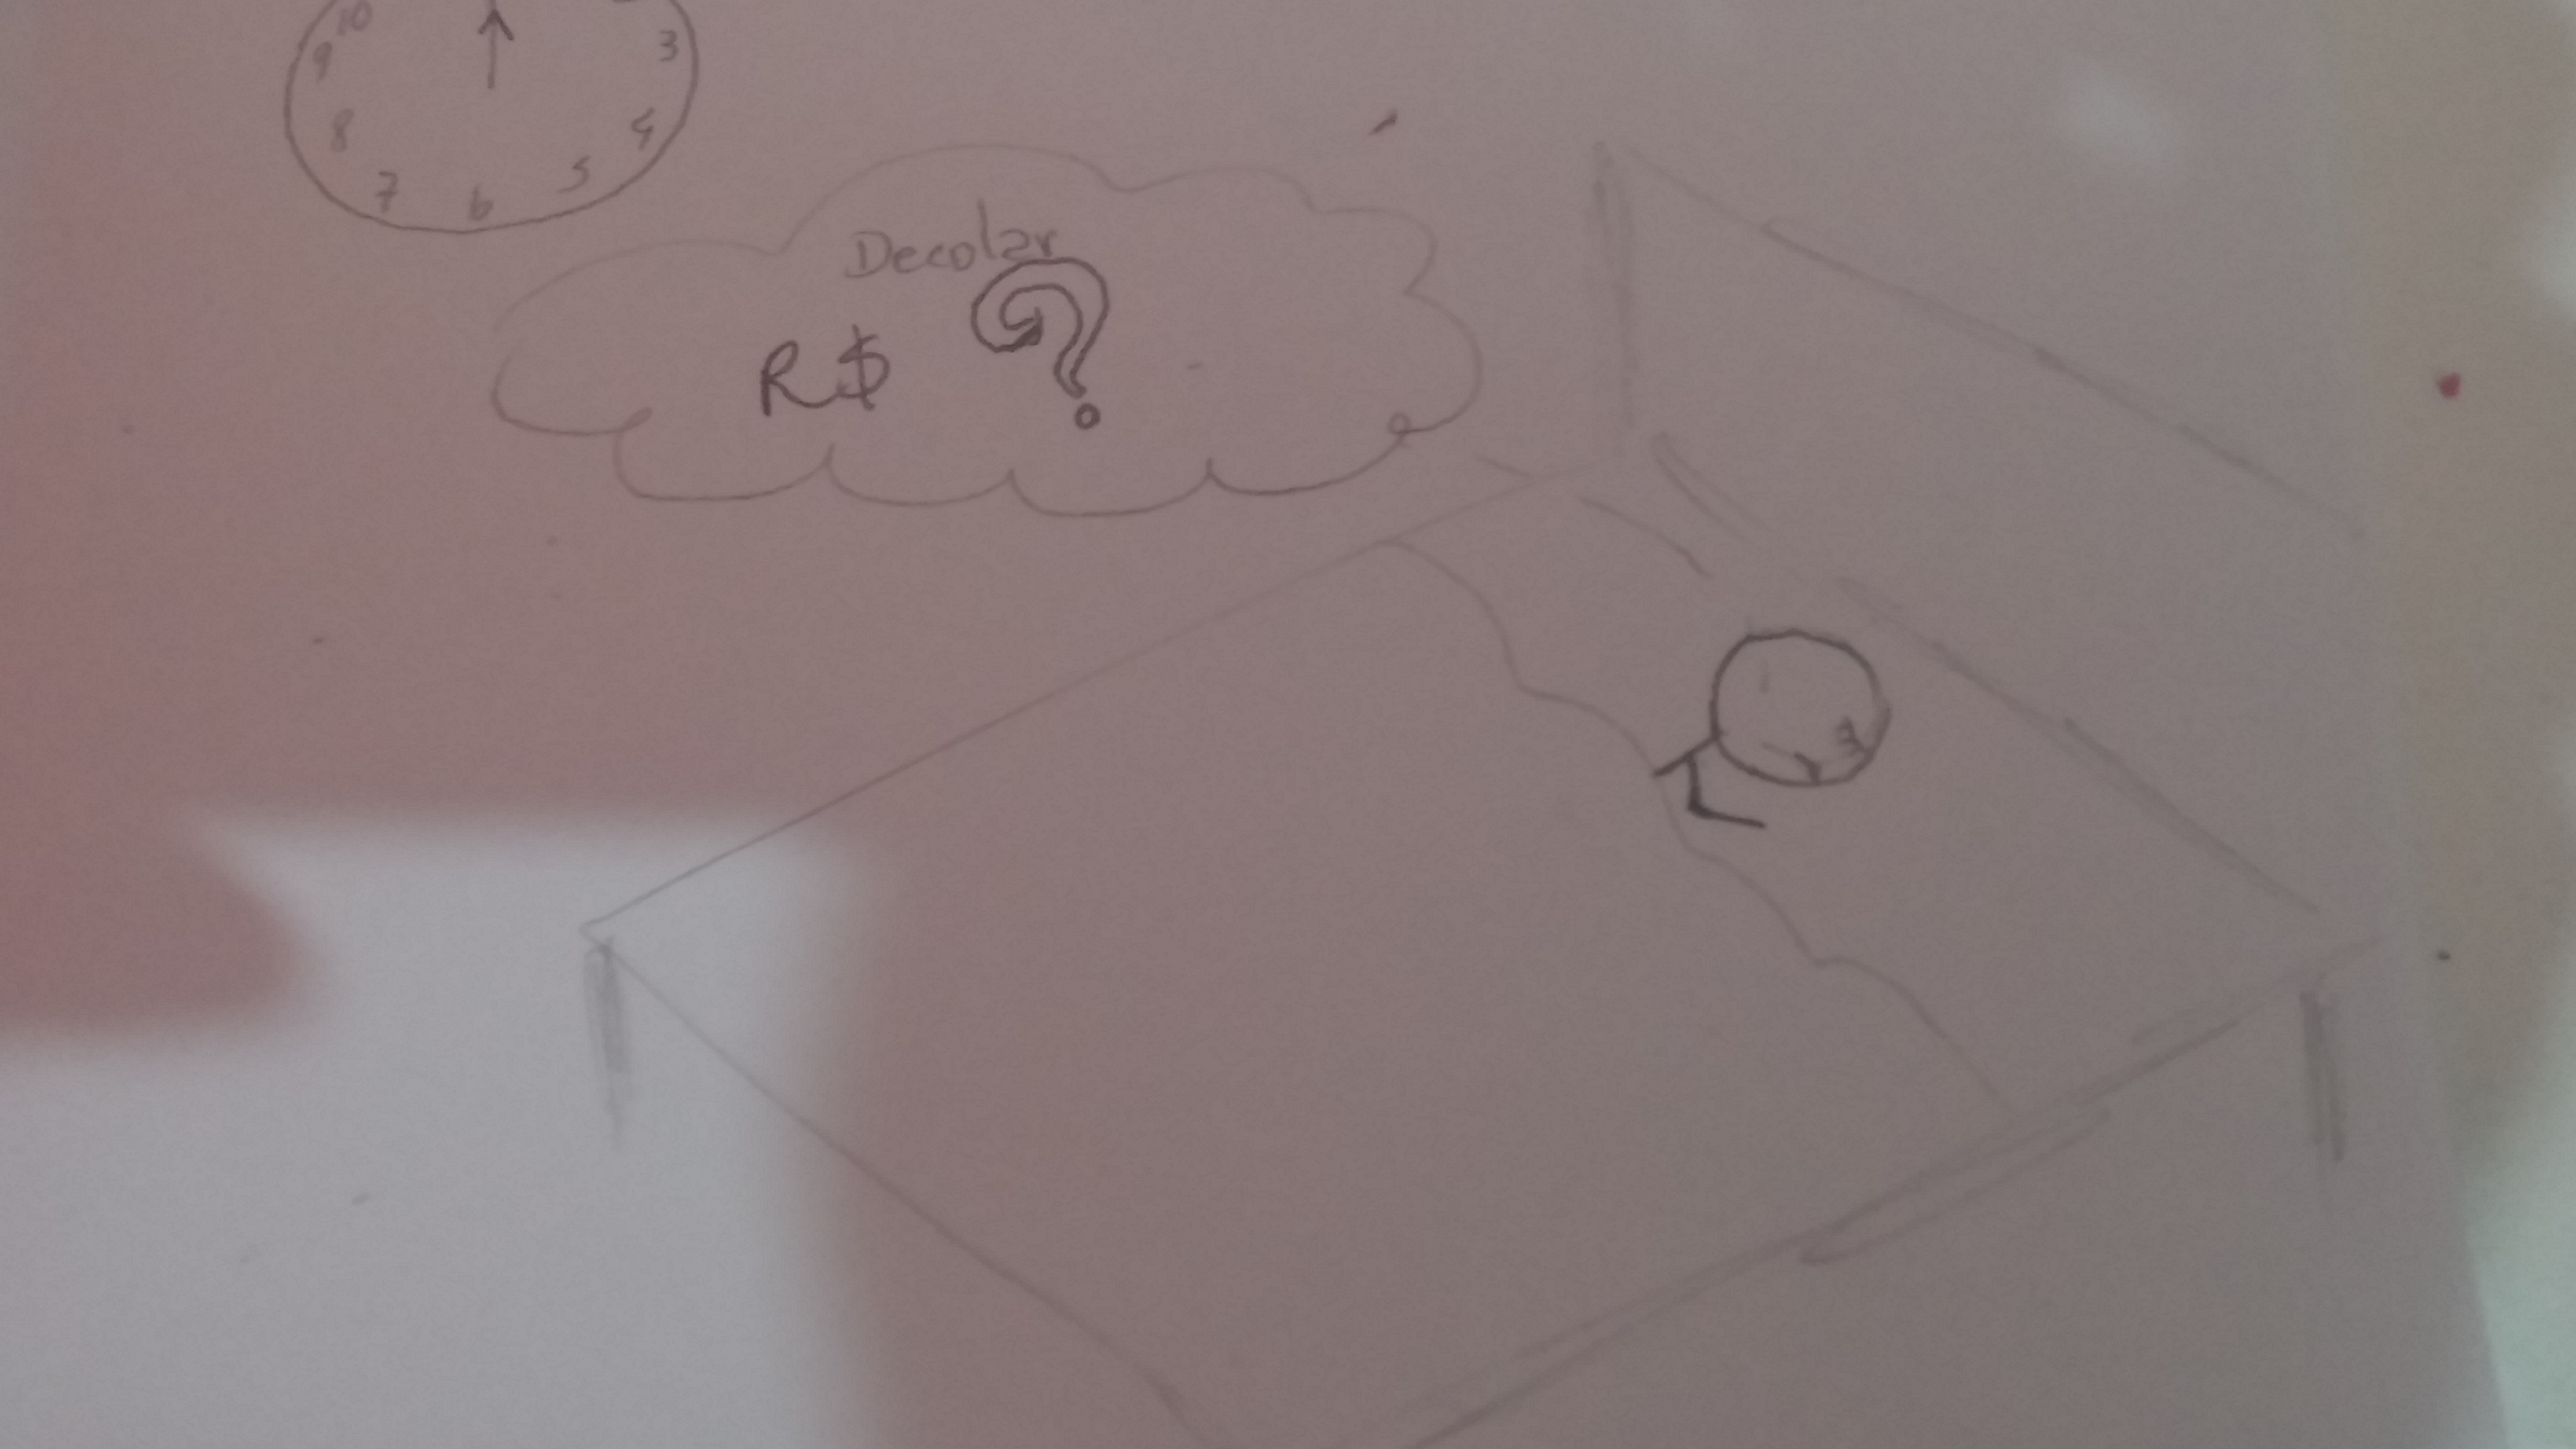
\includegraphics[keepaspectratio=true,scale=0.65]{figuras/quadro2.eps}
		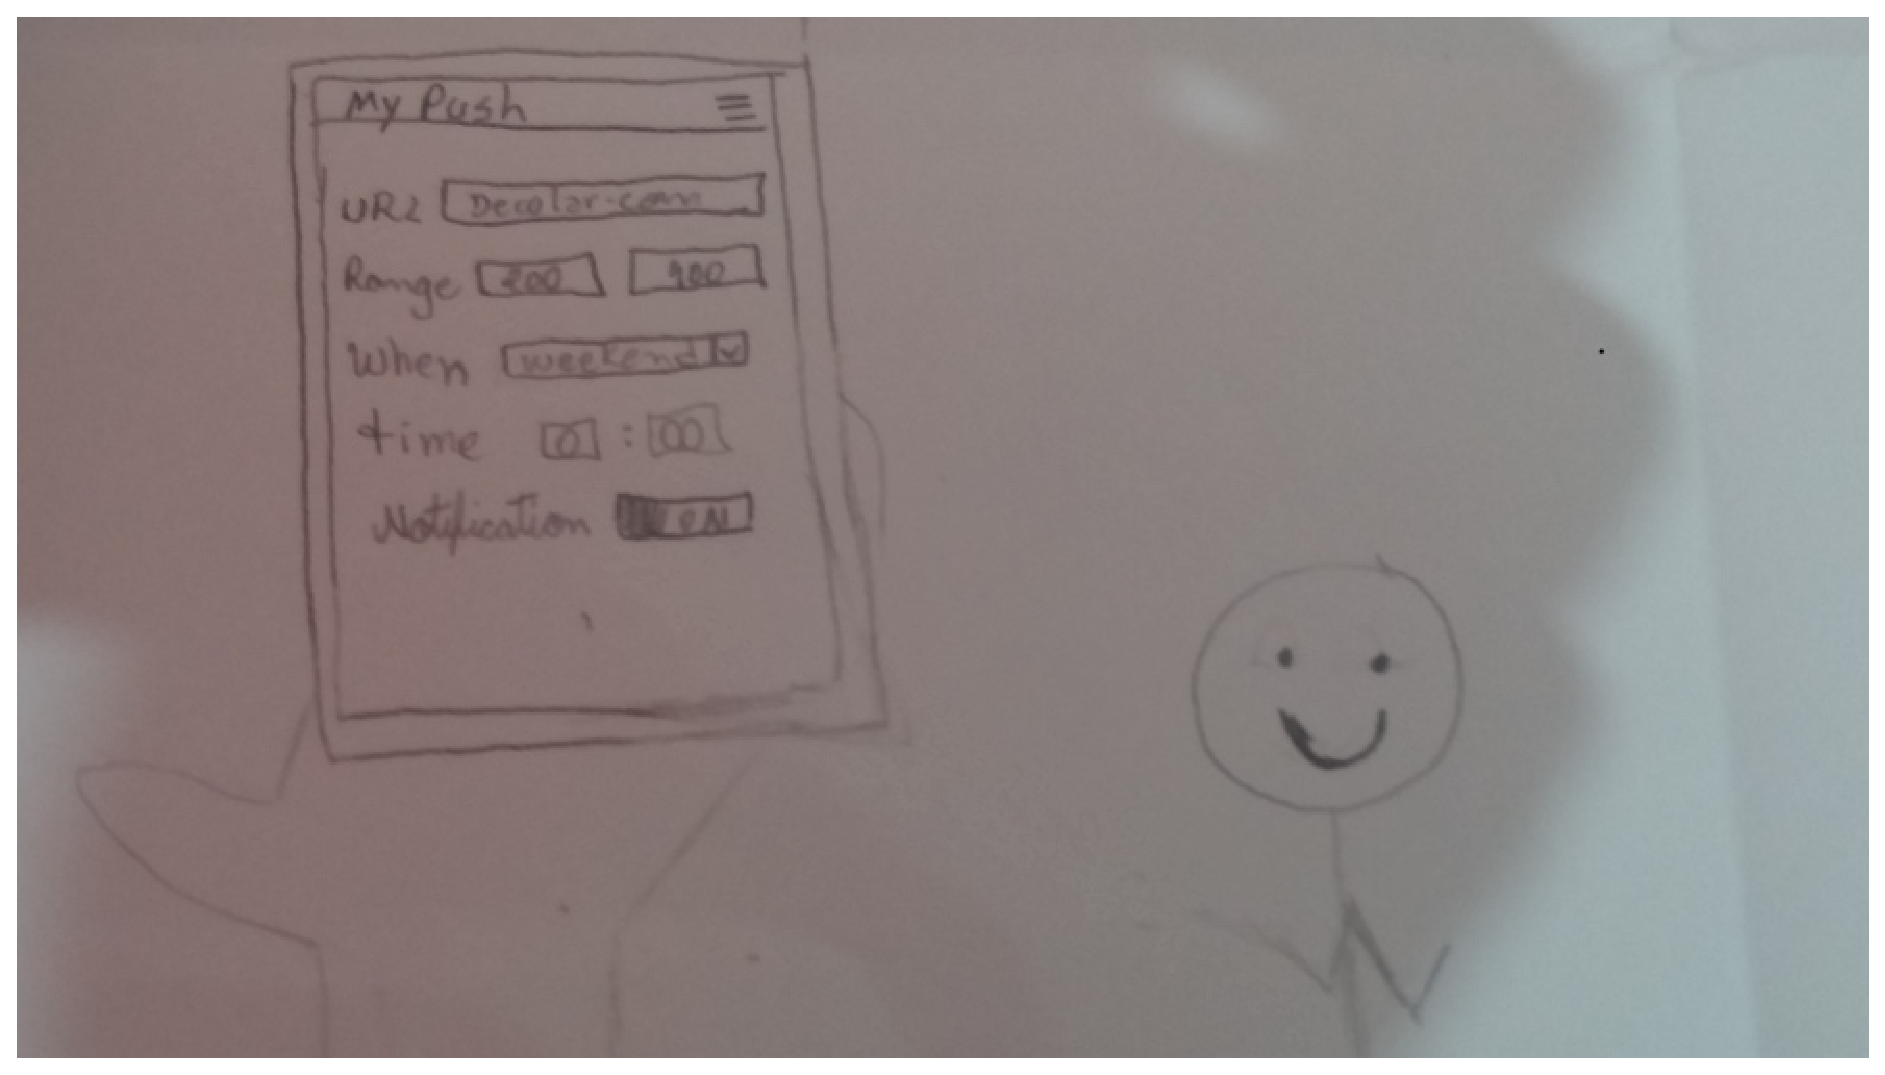
\includegraphics[keepaspectratio=true,scale=0.3]{figuras/quadro3.eps}
		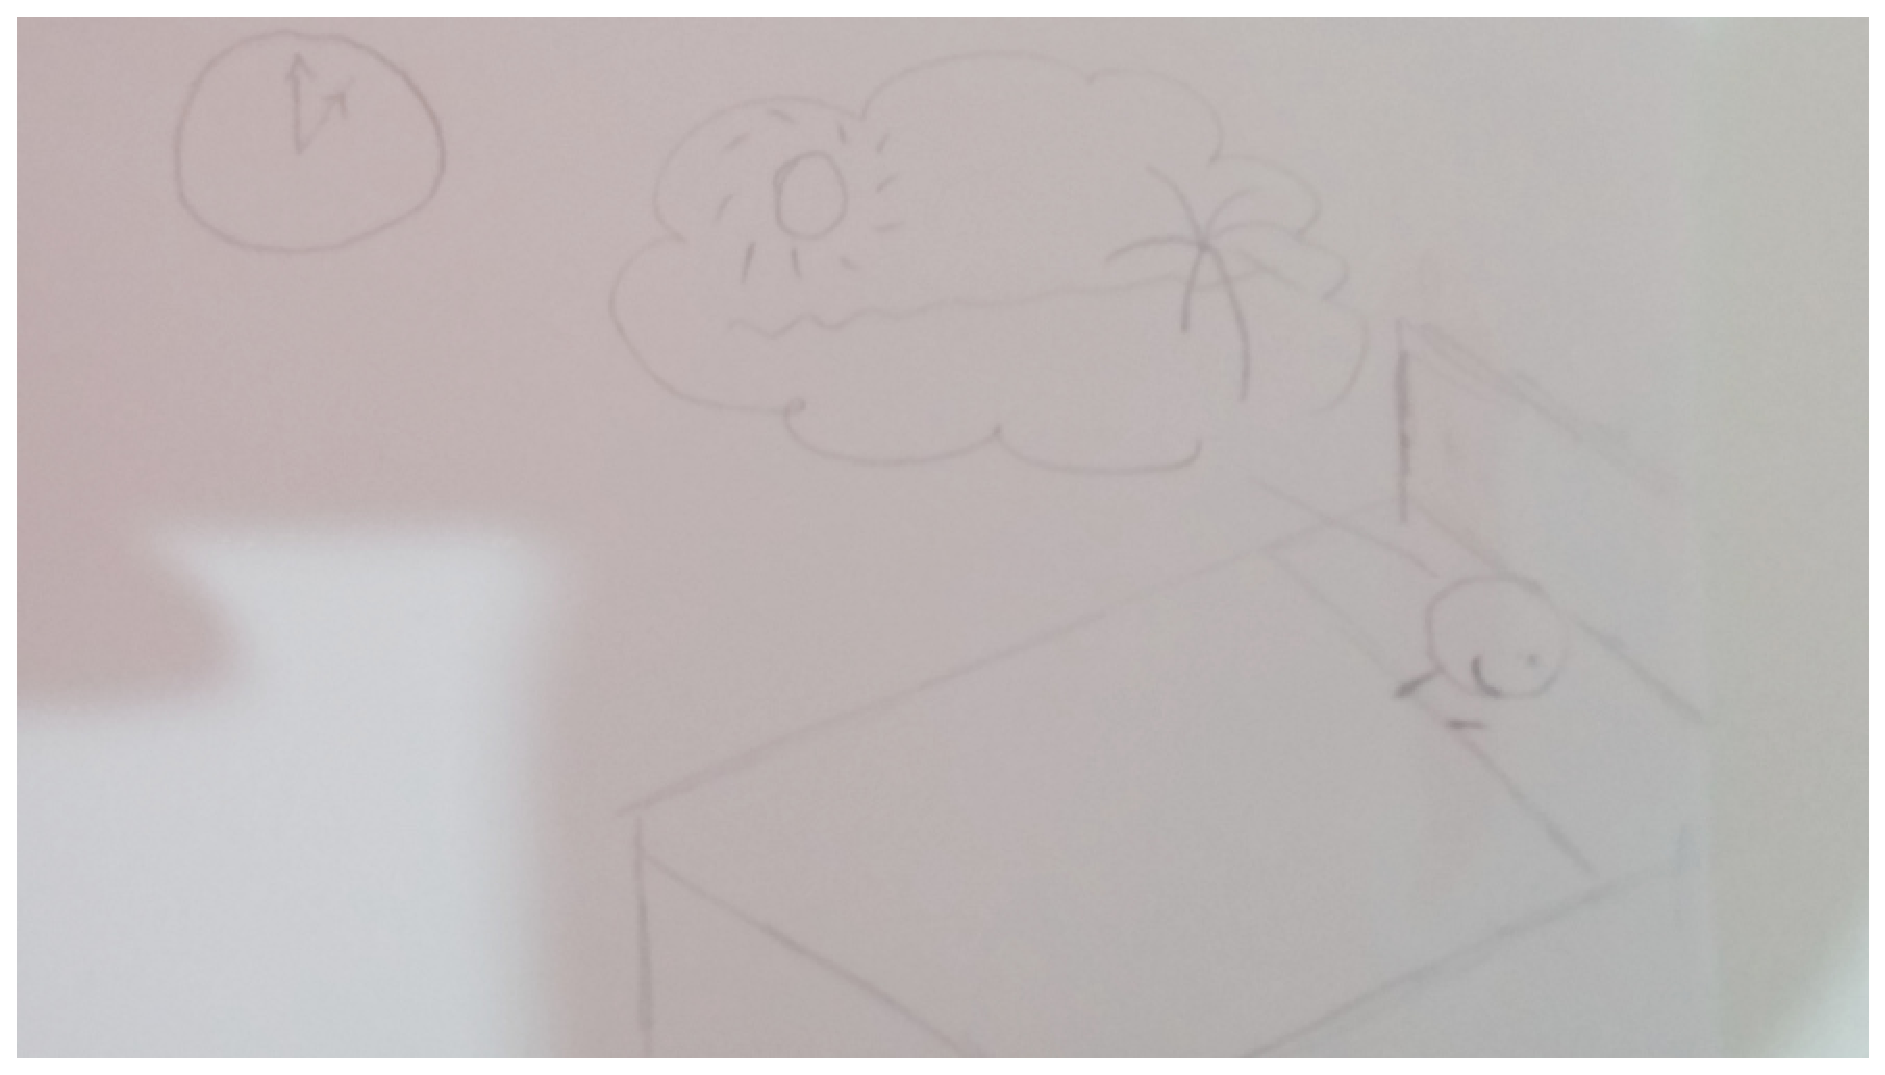
\includegraphics[keepaspectratio=true,scale=0.3]{figuras/quadro4.eps}
	\caption{Story Board - papel}
\end{figure}

\begin{figure}[h]
	\centering
	\label{fig02}
		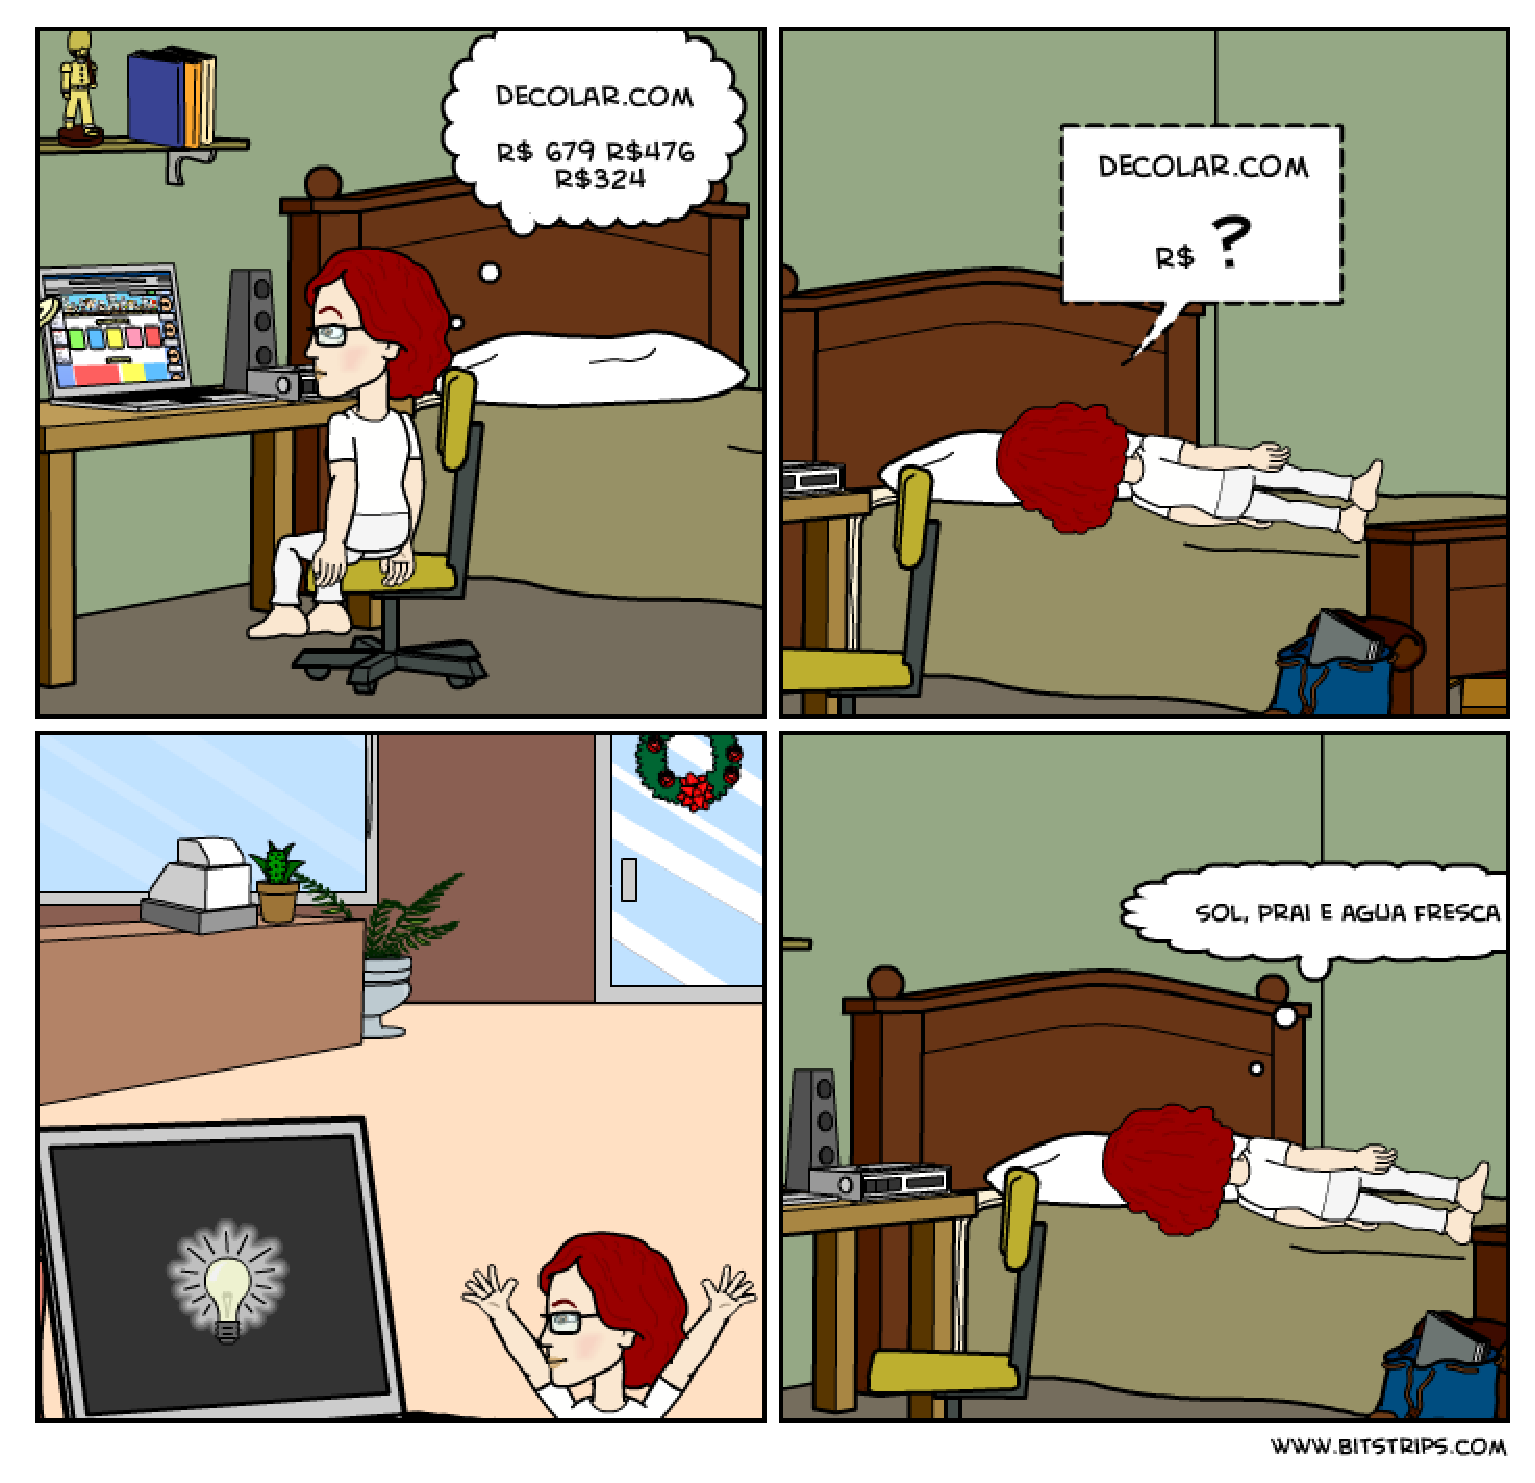
\includegraphics[keepaspectratio=true,scale=0.5]{figuras/ferramenta.eps}
		\caption{Story Board - ferramenta}
\end{figure}

\begin{figure}[h]
	\centering
	\label{fig03}
		\includegraphics[keepaspectratio=true,scale=0.075]{figuras/mockup/config_geral.eps}
		\includegraphics[keepaspectratio=true,scale=0.075]{figuras/mockup/config_site.eps}
		\includegraphics[keepaspectratio=true,scale=0.075]{figuras/mockup/cota_diaria.eps}
		\includegraphics[keepaspectratio=true,scale=0.075]{figuras/mockup/grafico.eps}
		\includegraphics[keepaspectratio=true,scale=0.075]{figuras/mockup/historico.eps}
		\includegraphics[keepaspectratio=true,scale=0.075]{figuras/mockup/menu.eps}
	\caption{Protótipo de papel validado}
\end{figure}
